\documentclass{standalone}

\usepackage{tikz}    

\begin{document}
		
	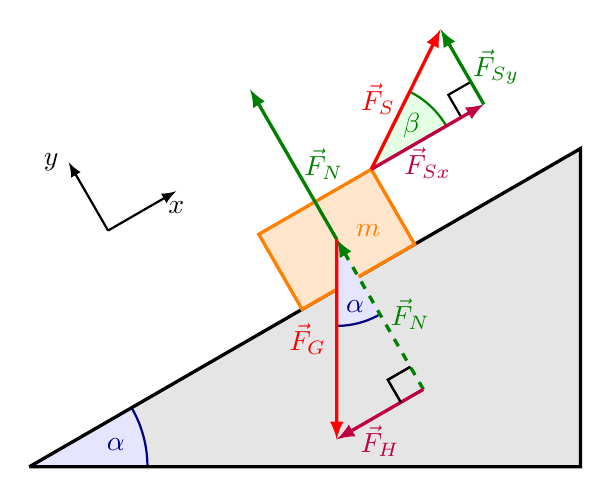
\begin{tikzpicture}
		
		
		%Raster im Hintergrund
		%\draw[step=1, gray, very thin] (0,0) grid (7,6);	

		%Grunddreieck	
		\draw [fill=gray!20] (0,0) -- (7,0) -- (7,4.04145) -- (0,0);
		
		%Winkel
		\filldraw[fill=blue!10, draw=blue!50!black, thick] (0,0) -- (1.5,0) arc(0:30:1.5) 
			node [midway, xshift=-10pt, yshift=-3, blue!50!black] {$\alpha$} {};
				
		\draw [very thick] (0,0) -- (7,0) -- (7,4.04145) -- (0,0);
				
		%Bezugssystem
		\begin{scope}[xshift=1cm, yshift=3cm, rotate=30, scale=1]
	    	%Länge x Achse
			\draw [-latex, thick] (0,0) -- ++(1,0) node[below] {$x$};
		
			%Länge y Achse
			\draw [-latex, thick] (0,0) -- ++(0,1) node[left] {$y$};
  		\end{scope}
  		%Alles was gedreht wurde (Masse m, Kräftevektoren, ...)
		\begin{scope}[xshift=3.464cm, yshift=2cm, rotate=30, scale=1.1]

			\coordinate (A) at (0.75,0.5);
			\coordinate (B) at (0.75,-1.5);
			
			%Rechteck
			\draw [fill=orange!20!white] (0,0) rectangle (1.5,1);
			\draw [orange, very thick] (0,0) rectangle (1.5,1) node [midway, right, xshift=3pt, yshift=3pt] {$m$} {} ;
			
			%Vektoren Kraft-Seil
			\begin{scope}[xshift=1.5cm, yshift=1cm, rotate=0, scale=1]
    			\begin{scope}[xshift=0cm, yshift=0cm, rotate=0, scale=1]
    				\filldraw[fill=green!10, draw=green!50!black, thick] (0,0) -- (1,0) arc(0:33.6900:1) 
    					node [midway, left, xshift=0pt, yshift=-7, green!50!black] {$\beta$} {};
    			\end{scope}
    			\coordinate (C) at (1.5,0);
				\coordinate (D) at (1.5,1);
				%Rechter Winkel
				\draw [thick](1.2,0) -- (1.2,0.3) -- (1.5,0.3);
    			\draw [-latex, very thick, purple] (0,0) -- ++ (C) node [midway, below] {$\vec{F}_{Sx}$} {};
				\draw [-latex, very thick, green!50!black] (C) -- ++ (0,1) node [midway, right] {$\vec{F}_{Sy}$} {};
				\draw [-latex, very thick, red] (0,0) -- ++ (D) node [midway, left] {$\vec{F}_S$} {};
				%Rechter Winkel
    			  
    		\end{scope}	
			
			%Vektoren FN, FG, FH
    		
    		\begin{scope}[xshift=0cm, yshift=0, rotate=0, scale=1]
    			\coordinate (A) at (0.75,0.5);
				\coordinate (B) at (0.75,-1.5);
    			\begin{scope}[xshift=0.75cm, yshift=0.5cm, rotate=-120, scale=1]
    				\filldraw[fill=blue!10, draw=blue!50!black, thick] (0,0) -- (1,0) arc(0:30:1) 
    					node [midway, above, xshift=-1.5pt, yshift=0, blue!50!black] {$\alpha$} {};
    			\end{scope}
    			%Rechter Winkel
    			\draw [thick](0.45,-1.5) -- (0.45,-1.2) -- (0.75,-1.2);  
    			\draw [-latex, very thick, dashed, green!50!black] (B) -- (A) node [midway, right] {$\vec{F}_N$} {};
				\draw [-latex, very thick, green!50!black] (A) -- ++(0,2) node [midway, right] {$\vec{F}_N$} {};
    			\draw [-latex, very thick, purple] (B) -- ++(-1.1547,0) node [midway, below] {$\vec{F}_H$} {};
    			\draw [-latex, very thick, red] (A) -- ++(-1.1547,-2) node [midway, left] {$\vec{F}_G$} {};
    			%Rechter Winkel
    			\draw [thick](0.45,-1.5) -- (0.45,-1.2) -- (0.75,-1.2);  
    		\end{scope}		    		
  		\end{scope}
		
	\end{tikzpicture}
\end{document}
